%%%%%%%%%%%%%%%%%%%%%%%%%%%%%%%%%%%%%%%%%%%%%%%%%%%%%%%%%%%%%%%%%%%%%
%%                                                                 %%
%% Please do not use \input{\dots} to include other tex files.       %%
%% Submit your LaTeX manuscript as one .tex document.              %%
%%                                                                 %%
%% All additional figures and files should be attached             %%
%% separately and not embedded in the \TeX\ document itself.       %%
%%                                                                 %%
%%%%%%%%%%%%%%%%%%%%%%%%%%%%%%%%%%%%%%%%%%%%%%%%%%%%%%%%%%%%%%%%%%%%%

%%\documentclass[referee,sn-basic]{sn-jnl}% referee option is meant for double line spacing

%%=======================================================%%
%% to print line numbers in the margin use lineno option %%
%%=======================================================%%

%%\documentclass[lineno,sn-basic]{sn-jnl}% Basic Springer Nature Reference Style/Chemistry Reference Style

%%======================================================%%
%% to compile with pdflatex/xelatex use pdflatex option %%
%%======================================================%%

%%\documentclass[pdflatex,sn-basic]{sn-jnl}% Basic Springer Nature Reference Style/Chemistry Reference Style

%%\documentclass[sn-basic]{sn-jnl}% Basic Springer Nature Reference Style/Chemistry Reference Style
\documentclass[sn-mathphys]{sn-jnl}% Math and Physical Sciences Reference Style
%%\documentclass[sn-aps]{sn-jnl}% American Physical Society (APS) Reference Style
%%\documentclass[sn-vancouver]{sn-jnl}% Vancouver Reference Style
%%\documentclass[sn-apa]{sn-jnl}% APA Reference Style
%%\documentclass[sn-chicago]{sn-jnl}% Chicago-based Humanities Reference Style
%%\documentclass[sn-standardnature]{sn-jnl}% Standard Nature Portfolio Reference Style
%%\documentclass[default]{sn-jnl}% Default
%%\documentclass[default,iicol]{sn-jnl}% Default with double column layout

%%%% Standard Packages
%%<additional latex packages if required can be included here>
%%%%

%%%%%=============================================================================%%%%
%%%%  Remarks: This template is provided to aid authors with the preparation
%%%%  of original research articles intended for submission to journals published
%%%%  by Springer Nature. The guidance has been prepared in partnership with
%%%%  production teams to conform to Springer Nature technical requirements.
%%%%  Editorial and presentation requirements differ among journal portfolios and
%%%%  research disciplines. You may find sections in this template are irrelevant
%%%%  to your work and are empowered to omit any such section if allowed by the
%%%%  journal you intend to submit to. The submission guidelines and policies
%%%%  of the journal take precedence. A detailed User Manual is available in the
%%%%  template package for technical guidance.
%%%%%=============================================================================%%%%

\jyear{2023}%

%% as per the requirement new theorem styles can be included as shown below
\theoremstyle{thmstyleone}%
\newtheorem{theorem}{Theorem}%  meant for continuous numbers
%%\newtheorem{theorem}{Theorem}[section]% meant for sectionwise numbers
%% optional argument [theorem] produces theorem numbering sequence instead of independent numbers for Proposition
\newtheorem{proposition}[theorem]{Proposition}%
%%\newtheorem{proposition}{Proposition}% to get separate numbers for theorem and proposition etc.

\theoremstyle{thmstyletwo}%
\newtheorem{example}{Example}%
\newtheorem{remark}{Remark}%

\theoremstyle{thmstylethree}%
\newtheorem{definition}{Definition}%

\raggedbottom
%%\unnumbered% uncomment this for unnumbered level heads




% JAIME: this is to hide font size warnings
\usepackage{anyfontsize}

% JAIME: For 1e-10 notation
\usepackage{siunitx}


\begin{document}

\title[Predicting Spotify Audio Features from Last.fm Tags]{Predicting Spotify Audio Features from Last.fm Tags}

%%=============================================================%%
%% Prefix	-> \pfx{Dr}
%% GivenName	-> \fnm{Joergen W.}
%% Particle	-> \spfx{van der} -> surname prefix
%% FamilyName	-> \sur{Ploeg}
%% Suffix	-> \sfx{IV}
%% NatureName	-> \tanm{Poet Laureate} -> Title after name
%% Degrees	-> \dgr{MSc, PhD}
%% \author*[1,2]{\pfx{Dr} \fnm{Joergen W.} \spfx{van der} \sur{Ploeg} \sfx{IV} \tanm{Poet Laureate}
%%                 \dgr{MSc, PhD}}\email{iauthor@gmail.com}
%%=============================================================%%

\author*[1]{\fnm{Jaime} \sur{Ramírez Castillo}}\email{Jaime.Ramirez@alu.uclm.es}

\author[1]{\fnm{M. Julia} \sur{Flores}}\email{Julia.Flores@uclm.es}
\equalcont{These authors contributed equally to this work.}


\affil[1]{\orgdiv{Departamento de Sistemas Informáticos}, \orgname{Universidad de Castilla-La Mancha}, \orgaddress{\street{Campus universitario s/n}, \city{Albacete}, \postcode{02071}, \country{Spain}}}


%%==================================%%
%% sample for unstructured abstract %%
%%==================================%%

\abstract{
    In this paper, we discuss a number of experiments to analyze the
    suitability of music label representations to predict certain audio features,
    such as danceability, loudness, or acousticness \dots
}


% TENSES: https://blog.wordvice.com/video-which-verb-tenses-should-i-use-in-a-research-paper/

%%================================%%
%% Sample for structured abstract %%
%%================================%%

% \abstract{\textbf{Purpose:} The abstract serves both as a general introduction to the topic and as a brief, non-technical summary of the main results and their implications. The abstract must not include subheadings (unless expressly permitted in the journal's Instructions to Authors), equations or citations. As a guide the abstract should not exceed 200 words. Most journals do not set a hard limit however authors are advised to check the author instructions for the journal they are submitting to.
%
% \textbf{Methods:} The abstract serves both as a general introduction to the topic and as a brief, non-technical summary of the main results and their implications. The abstract must not include subheadings (unless expressly permitted in the journal's Instructions to Authors), equations or citations. As a guide the abstract should not exceed 200 words. Most journals do not set a hard limit however authors are advised to check the author instructions for the journal they are submitting to.
%
% \textbf{Results:} The abstract serves both as a general introduction to the topic and as a brief, non-technical summary of the main results and their implications. The abstract must not include subheadings (unless expressly permitted in the journal's Instructions to Authors), equations or citations. As a guide the abstract should not exceed 200 words. Most journals do not set a hard limit however authors are advised to check the author instructions for the journal they are submitting to.
%
% \textbf{Conclusion:} The abstract serves both as a general introduction to the topic and as a brief, non-technical summary of the main results and their implications. The abstract must not include subheadings (unless expressly permitted in the journal's Instructions to Authors), equations or citations. As a guide the abstract should not exceed 200 words. Most journals do not set a hard limit however authors are advised to check the author instructions for the journal they are submitting to.}

\keywords{Music information retrieval, Artificial intelligence}

%%\pacs[JEL Classification]{D8, H51}

%%\pacs[MSC Classification]{35A01, 65L10, 65L12, 65L20, 65L70}

\maketitle

\section{Introduction}\label{sec1}

Music information retrieval (MIR) is an interdisciplinary research field that encompasses the extraction,
processing, and knowledge discovery of information contained in music.
MIR research covers a wide range of applications and intersects with other areas, such as computer science, signal processing, musicology, and sociology.
Examples of MIR applications are recommendation systems, music classification,
music source separation, and music generation, among others \cite{ramirez2020machine}.

MIR applications often attempt to extract information from the music audio signal,
although analyzing associated metadata is also a common practice.
Audio signals are typically preprocessed and transformed into intermediate formats, such as frequency-based signal representations (e.g. spectrograms),
and sets of hand-crafted audio features, which are typically engineered by using domain knowledge (e.g. MFCC, rhythm, or tonal descriptors).

The metadata associated to a music piece is available in multiple formats.
Editorial information or lyrics, for example, are mostly available in text format.
The ability to process images or videos is also required, for example, for analyzing album artwork, or music videos.

Depending on the specific MIR application, researchers or practitioners expect different output values.
Applications that extract audio features typically return audio descriptors, namely values related to the tempo, the key, or the sample rate, among others.
Open source libraries such as \emph{Librosa}\footnote[1]{https://librosa.org/} 
and \emph{Essentia}\footnote[2]{https://essentia.upf.edu/index.html} offer methods to extract these values.
Other applications might produce higher-level values, for example, by using machine learning techniques
that estimate the emotion that a track induces, or the music genre of this track.

Among potentially useful input and output values, research has proved Spotify audio features and Last.fm tags to be significant values to characterize music.
Spotify audio features capture high-level information about the music signal,
such as energy, danceability, or valence, among others.
Last.fm tags are text labels that users associate to songs, artists, and albums via the Last.fm social platform.

Both Spotify audio features and Last.fm tags have been used as input data mostly for classification tasks, such as music genre recognition,
where, given a set of Spotify audio features and/or Last.fm tags, the model estimates the music genre(s) of a particular track.
Previous studies, however, have not experimented with these values as target outputs, to the best of our knowledge.
This unexplored aspect reveals what we believe is a potential research opportunity in music analysis and recommendation.

In particular, this article focuses on predicting Spotify audio features, given a set of Last.fm tags.
By predicting Spotify audio features, we explore the relationship between the subjective perception captured by Last.fm tags, and the concrete musical features that Spotify computes.
This approach might help to identify patterns and hidden correlations between how music is perceived, consumed, and discovered.

Additionally, the predicted Spotify audio features could be used in recommendation systems to provide users with explainable recommendations.
Music recommendations are typically difficult to interpret from the perspective of the listener.
Users often get recommendations without meaningful explanations or justifications.
By predicting Spotify features as an intermediate step in the recommendation pipeline, we could use these features to explain users why the algorithm suggests a particular track.
This process could be part of an explainable recommendation pipeline, where users enter a set of tags,
and as a result they get the predicted audio features, the closest tracks to those features (as recommended tracks), and the distance values between each track and the predicted features.

% The idea is, given a set of tags, to predict a set of audio features that a hypothetic track would exhibit.
% Then, we could build a track selection algorithm that selects actual tracks that are the closest to the predicted audio features.
% This process could be part of an explainable recommendation pipeline, where users enter a set of tags, and they recieve the predicted audio features, the closest tracks to those features, and the distance values between each track and the predicted features.

In the remainder of the article, we explain the data gathering and preparation process, as well as the data input formats and varios models.
We will explore various models for the same track and provide insights on how accurately the prediction can be, by using only Last.fm tags.
\textcolor{red}{UNDER DEVELOPMENT}

\section{Data Sources}

\subsection{Last.fm Tags}

Last.fm is an online music community where users keep track of their music listening habits.
Users apply tags to artists, tracks, and albums to categorize and describe music from their own perspective, which
implies that the Last.fm tags space does not fit into any structured ontology or data model.
A tag can refer to any aspect that users consider to be a valid descriptor, such as genre,
emotion, or user listening context.

For nearly two decades, many music aficionados have collectively contributed their own unique, personal interpretation, opinions and feelings
as tags in Last.fm.
Although many of these tags are single-worded descriptors (e.g \emph{rock}, \emph{dance}, or \emph{happy}),
users also use short sentences to describe music, such as \emph{I like this track}, or \emph{on the beach}.

Tags are available via the Last.fm API.

\subsection{Spotify Audio Features}

Spotify, one of the leaders in the music streaming industry, provides information about the tracks in their catalog via the Spotify developers API.
Among the different data entities exposed, the API provides access to the \emph{Audio Features} for each track.

The Spotify audio features are numerical values that represent high-level audio information computed from a specific
track. These values characterize a track, musically speaking,
by measuring musical aspects that, in many of these features, are related to the user perspective or recommendation factors.
For example, a danceability value of 0.95 means
that a particular song is highly suitable for dancing.

The features provided by the Spotify API are listed in
Table \ref{table:spotify-features}.
While Spotify provides a description of the audio features.
How they compute or estimate these values is not publicly available.
The reader can find further details about each feature in the Spotify API documentation\footnote[5]{
      \url{https://developer.spotify.com/documentation/web-api/reference/\#/operations/get-audio-features}
}.

\begin{table}[h!]
      \centering
      \caption{Spotify audio features. These features provide high-level musical information about a track.} \label{table:spotify-features}
      \begin{tabular}{p{0.3\linewidth}p{0.6\linewidth}}
          \toprule
          \bfseries \textbf{Feature name} & \textbf{Description} \\
          \midrule
          \textbf{acousticness} & The track is acoustic. From 0 to 1 \\
          \textbf{danceability} & The track encourages (or is adequate for) dancing. From 0 to 1 \\
          \textbf{duration\_ms}  &  Duration in milliseconds \\
          \textbf{energy}  &  The track is perceived as energetic. From 0 to 1\\
          \textbf{instrumentalness}  &  The track is instrumental. From 0 to 1 \\
          \textbf{key}  &  Key categories encoded as integers. From C (0) to 11 \\
          \textbf{liveness}  &  The audience is audible. From 0 to 1\\
          \textbf{loudness}  &  In decibels. From -60 to 0 \\
          \textbf{mode}  & Major (1) or minor (0) \\
          \textbf{speechiness}  & Does the track contain speeches? From 0 to 1 \\
          \textbf{tempo}  & In beats per minute (BPM) \\
          \textbf{valence} & How happy is the track (BPM). From 0 to 1 \\
          \bottomrule
      \end{tabular}
  \end{table}


\section{Related Research}

The objective of this study is to predict Spotify audio features from Last.fm tags, so the objective of this section is to
explore existing literature that is related to the problem and review the facts that are important or relevant for our experimentation.

The use of Last.fm tags and Spotify audio features has been common and prolific in studies
that have applied machine learning to resolve MIR challenges.

An important concept to consider is the arousal-valence cuadrants, present in music emotion recognition, 
related to some studies that will be reviewed in the following sections, and also related to the valence and energy
Spotify audio features.

\subsection{Last.fm Tags}

In the last decade, researchers have studied the use of Last.fm tags in classification and regression tasks.
Last.fm tags have been a popular source of metadata for MIR tasks,
because they potentially contain subjective information related to the genre, mood, and style of music,
and might be used to characterize certain features of a music piece.
Additionally, Last.fm tags constitute a useful source of input knowledge when the audio signal is not available,
for example, due to copyright limitations.


Several studies have used Last.fm to predict music sentiment, mood, and even audio features.
For example, Laurier et al. analyzed how Last.fm tags categorize mood.
In their study, they created a semantic mood space based on Last.fm tags \cite{laurier2009music}.

% This study predicts Spotify features from Predictor Variables – Determinants of Music-Selection Behavior
% https://www.static.tu.berlin/fileadmin/www/10002020/Dokumente/Abschlussarbeiten/Karnop_MasA.pdf

% == Excerpt taken from one of our references vvvvvvv
% For example, tags such as "acoustic", "live", and "instrumental" have been
% shown to be good predictors of the energy and danceability of a track.
% Similarly, tags such as "happy," "sad," and "angry" have been used
% to predict the valence and arousal of a track.

{\c{C}}ano and Morisio performed an analysis of Last.fm tags to create a dataset of music
lyrics annotated with Last.fm tags.
In the creation process, they concluded that Last.fm tags are mostly related to music genre
and positive moods \cite{ccano2017music}.

In a similar direction, Bod{\'o} and Szil{\'a}gyi generated a dataset for lyrics genre classification
by combining the Last.fm with \emph{MusicBrainz} data \cite{bodo2018connecting}.
MusicBrainz is an online database of music editorial metadata\footnote[1]{https://musicbrainz.org/}.

Although different datasets that contain Last.fm tags have been created, so far,
the \emph{Last.fm dataset}\footnotemark[2] has been the most widely used in research.
This dataset is a complementary dataset of the Million Song Dataset (MSD) \cite{Bertin-Mahieux2011}.

\footnotetext[2]{Last.fm dataset, the official song tags and song similarity collection for the Million Song
Dataset, available at: http://millionsongdataset.com/lastfm.}

In general, these studies confirm the possibility of extracting knowledge from Last.fm tags.

\textcolor{red}{We introduced this section talking about machine learning but only refeferred to studies
that use Last.fm tags in exploration and data set creation}

\subsection{Spotify Audio Features}

Historically, the Spotify audio features features were called the \emph{Echo Nest audio features}.
\emph{The Echo Nest} was an online music intelligence platform that provided users and clients with music analysis services.
Among these services, the Echo Nest offered a database and an API to retrieve audio features for each of the tracks in the database \footnote[3]{https://en.wikipedia.org/wiki/The\_Echo\_Nest}.
Spotify acquired the Echo Nest in 2014.
As a result, the Echo Nest API was eventually deactivated and Spotify migrated these audio features to the Spotify API.

Nowadays, the two terms can be found in published research.
Whereas the most recent studies refer to the Spotify audio features,
earlier studies use the Echo Nest denomination.

Regardless of the term used, the features remain the same.
These features are a set of high-level descriptors, such as energy and danceability,
which are related to the audio but also to the listeners perception.

Similarly to Last.fm, Spotify (or Echo Nest) audio features are commonly present in MIR research.
For example, Wang and Horv{\'a}t used  these audio features to study the differences 
between male and female artists \cite{wang2019gender}.
\textcolor{red}{Y que consiguieron?}

Jamdar et al. used Echo Nest audio features, combined with lyrics data to classify songs into emotion tags.
These classes were first defined based on a Last.fm tags emotion mapping \cite{jamdar2015emotion}.

Similarly, Non-negative Matrix Factorization was applied in combination with EchoNest audio features
for song recommendations \cite{benzi2016song}.

Panda and Redinho explore the use of Spotify high-level features applied to Music Emotion Recognition (MER) \cite{panda2021does}.
In particular, they identify that the energy, valence, and acousticness values, provided by the Spotify API,
are highly relevant for emotion classification.
They also achieve better performance on MER models by using their own top-100 features, and they determine that,
although these three Spotify features are relevant in terms of characterizing emotion,
more features are needed to effectively recognize emotion.
Another interesting observation of this study is the the identification of energy as a surrogate of arousal valence


In general, Spotify audio features have been used as predictive input variables.
We, to the best of our knowledge, are unaware of studies that use these features as target variables,
or studies that have addressed the problem of audio features regression, based solely on Last.fm tags.


Similarly to Last.fm tags, Spotify audio features can be found in a number of datasets.
Publicly available datasets of Spotify audio features can be found online,
as a result of open-source and research communities collecting data from the Spotify API and publishing the results.
It is unclear, however, whether these published datasets completely meet the Spotify API terms of service.

For example, \emph{P4kxspotify} is a publicly available dataset that combines music review texts with Spotify audio features.
The dataset creators argue that, although the terms of service prohibits scraping, their work is ethical \cite{pinter2020p4kxspotify}.




Another publicly available dataset is the \emph{Spotify Audio Features} Kaggle dataset\footnote[4]{https://www.kaggle.com/datasets/tomigelo/spotify-audio-features}.
This dataset contains more than 116,000 unique tracks, and includes audio features for each track.

For this reason, we chose to generate our own dataset.

% Another dataset created from the Spotify API and published to Kaggle:
% https://www.kaggle.com/datasets/andrewmvd/spotify-playlists


% TODO: move explanation to the experiment section.
% \subsubsection{Machine Learning Models}

% Several studies have explored the use of machine learning
% models to predict audio features from audio metadata, such as Last.fm tags.
% % which studies use Last.fm tags as parameters?

% The experiments conduced in this study used two classical regression models,
% Boosted tree regressor and Bayesian ridge regressor.
% These two machine learning models that have been widely used in MIR. % is this true? (refs)

% Boosted tree regressor is a decision tree-based model that sequentially
% adds weak learners to the model to improve its performance.
% Bayesian ridge regressor, on the other hand,
% is a probabilistic model that uses Bayesian inference to estimate
% the parameters of the model.

% Additionally, language models, such as GTP-2 have shown promising results in various
% natural language processing (NLP) and generation.

% In this particular study, GTP-2 has been fine-tuned for regression tasks,
% and has shown good performance in predicting audio features from metadata.

% This paper aims to apply the boosted tree regressor,
%  Bayesian ridge regressor, and GTP-2 models to predict Spotify audio features from Last.fm tags.
% The experiments compare the performance of these models and evaluate their effectiveness
% in predicting various audio features.
% The results of these experiments will provide insights into
% the use of different machine learning models for MIR tasks
% and can have practical applications
% in music recommendation systems and genre or mood recognition.
%
%\textcolor{red}{To be Continued \dots }

\section{Generating a Dataset}

Before conducting experiments to predict audio features from tags,
we constructed a dataset of Last.fm tags and Spotify audio features, indexed by track, by gathering the data from the Last.fm and Spotify APIs.

The tracks were selected from the listening history of a single user.

\subsection{A Single-user Dataset}

This work is scoped within our single-user research line \cite{ramirez2022user}.
In this area, we explore the development of music recommender systems that
characterize the music preferences and listening context only for a single user.
Therefore, we extracted the data from the
listening history of the corresponding author in Last.fm\footnote[5]{https://www.last.fm/user/jimmydj2000}.

By training our system in a single-user space, we also raise the following question: Is it possible to train
recommender systems, and in particular, user-centric systems, by using a single-user dataset?
Additionally, we wanted to explore the idea of mimicking the fact that each human perceives music individually.
If we train a system on data from different users, then the system would share the view of multiple individuals.

Using a single-user data set might sound counterproductive in a machine learning scenario, specially considering
how machine learning breakthroughs have attempted, and succeeded in many cases, to generalize in a particular problem.
This is not objective of this study, which explores how a machine learning model can represent the music consumption experience of a single human.
The model must be able to generalize, but only within the context of the user's musical taste, which be believe can be possible, given a sufficiently large listening history.


\subsection{Gathering Listening History and Tags from Last.fm}

Last.fm uses the term \emph{scrobble} to refer to the action of playing a track at a specific moment in time.
Last.fm started monitoring user listening activity with a desktop application called \emph{Scrobbler}.
Users used to install this application on their computers to monitor their activity on players such as Winamp or iTunes.
With the advent of music streaming services, the possibilities for users to scrobble their music habits expanded.
Integrations where developed to integrate the scrobbler into popular platforms,
such as Spotify, YouTube, or SoundCloud.
Mobile versions of the Scrobbler were also developed for Android and iOS devices, while open source initiatives flourished too\footnote[6]{https://github.com/elamperti/OpenWebScrobbler}.


For us, the first step to construct the dataset was to download the user listening activity.
We queried the Last.fm API to download the user{'}s scrobbling logs, reported from 2007 to 2022.
For each scrobble, we have gathered the following information:

\begin{itemize}
\item Playback timestamp
\item Track name
\item Artist name
\item Track tags
\end{itemize}

Last.fm maps each track (and artist) to a list of community-contributed tags.
For each track-tag mapping, Last.fm includes
a \emph{count} value, which indicates the popularity of the given tag for the track.
Last.fm normalizes this value in the 0-100 range, so the most popular tag for a track is tipically associated with a
count value of 100.
For example, if \emph{jazz} is the most popular tag for a track,
then the track might be probably associated to the following tuple \verb|(jazz, 100)|.

Users tipically listen to their favorite tracks several times,
so the amount of unique tracks played is smaller
than the number of track plays. In this case, the amount of
individual tracks listened in a 15-year period is about \num{20000} and the number of scrobblings is, approximately, \num{90000}.
Therefore, the user has listened to each song, approximately, \num{4.5} times on average.


\subsection{Gathering Spotify Audio Features}

After collecting the listening history and track tags from Last.fm, and identifying the unique
tracks that represent the user music collection, we used the Spotify API to
collect audio features for each one of the \num{20000} individual tracks.


The mapping between Last.fm and Spotify tracks was performed on an artist-track basis.
For each track, the artist and track name extracted from Last.fm were used as parameters of the Spotify Search API.
The Last.fm API provides a unique identifier, the \emph{MusicBrainz} ID.
The Spotify API, however, does not provide this value.

\subsection{Filtering Missing Values}

After retrieving audio features, we identified that the Spotify API had failed to provide audio features for a portion of the tracks.
Similarly, Last.fm also returned no tags for another subset of the tracks.
To prevent problems with missing values, we decided to filter out these tracks from the dataset.
After filtering tracks that were missing Last.fm tags or Spotify audio features,
the dataset resulted in \num{14009} samples.
Compared to the original \num{20000} unique tracks included in the listening history, approximately \num{6000} songs were missing either Spotify or Last.fm data.
In other words, about 70\% of the tracks in the user listening history included relevant information for the study.




\subsection{Dataset Comparison}

Considering that the data was gathered from a single user,
we explored the data to verify that the distribution of the Spotify audio features
was comparable to larger, and possibly more balanced, Spotify datasets.
In particular, we verified that the distribution of the features,
described in Table \ref{table:audio-features-stats} and Figure \ref{fig:audio-features-distribution},
was comparable to the distribution of the Spotify Audio Features Kaggle dataset.
Our dataset, which we call \emph{Last.fm Single-user} dataset, presents mean ($\mu$) and standard deviation($\sigma$) values that are comparable to the same values of the Spotify Audio Features Kaggle dataset,
as illustrated in Table \ref{table:audio-features-stats-kaggle}
and Figure \ref{fig:audio-features-distribution-kaggle}.

% Another dataset created from the Spotify API and published to Kaggle:
% https://www.kaggle.com/datasets/andrewmvd/spotify-playlists

\begin{table}[!ht]
      \begin{minipage}{.5\linewidth}
      \caption{Audio features description of the Last.fm Single-user dataset.}\label{table:audio-features-stats}
            \centering
                  \begin{tabular}{@{}lll@{}}
                  \toprule
                  Feature           & $\mu$ & $\sigma$ \\
                  \midrule
                  Danceability      & 0.60  & 0.19  \\
                  Energy            & 0.63  & 0.23  \\
                  Acousticness      & 0.22  & 0.30  \\
                  Instrumentalness  & 0.51  & 0.38  \\
                  Valence           & 0.44  & 0.28  \\
                  \botrule
                  \end{tabular}
      \end{minipage}
      \begin{minipage}{.5\linewidth}
      \caption{Audio features description of Spotify Audio Features Kaggle dataset.}\label{table:audio-features-stats-kaggle}%
            \centering
                  \begin{tabular}{@{}lll@{}}
                  \toprule
                  Feature           & $\mu$ & $\sigma$ \\
                  \midrule
                  Danceability      & 0.58   & 0.19  \\
                  Energy            & 0.57  & 0.26  \\
                  Acousticness      & 0.34  & 0.25  \\
                  Instrumentalness  & 0.22  & 0.36  \\
                  Valence           & 0.44  & 0.26  \\
                  \botrule
                  \end{tabular}
      \end{minipage}

\end{table}
% \begin{table}[h!]
%       \begin{center}

%       \end{center}
% \end{table}

\begin{figure}[h!]
      \centering
      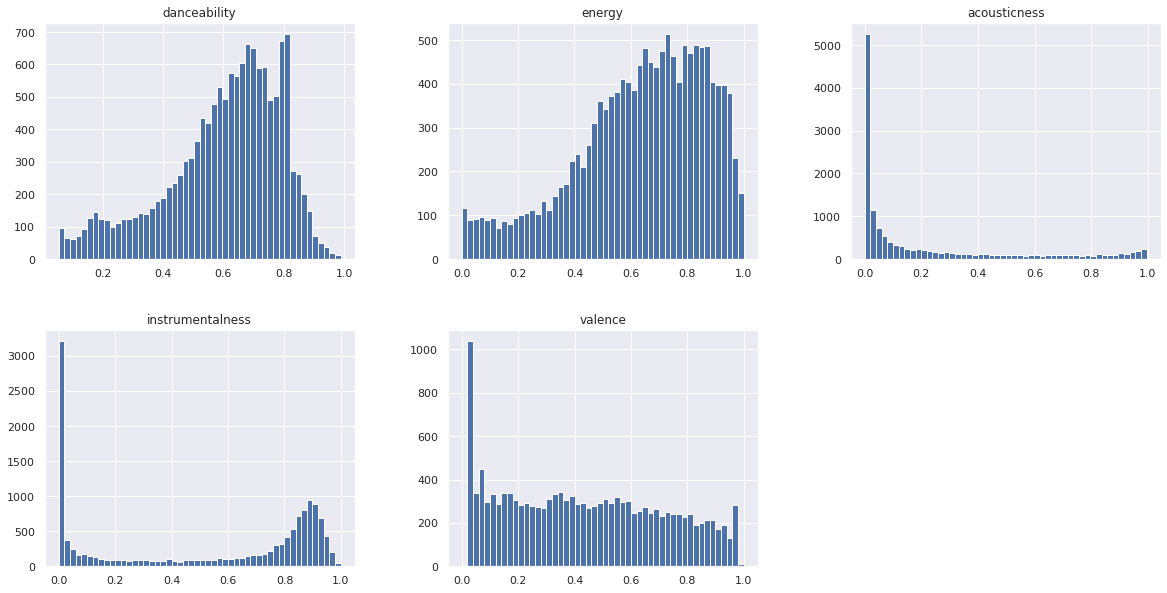
\includegraphics[width=\textwidth]{images/features-distribution.png}
      \caption{Distribution of audio features in the Last.fm Single-user dataset.}
      \label{fig:audio-features-distribution}
\end{figure}

\begin{figure}[h!]
      \centering
      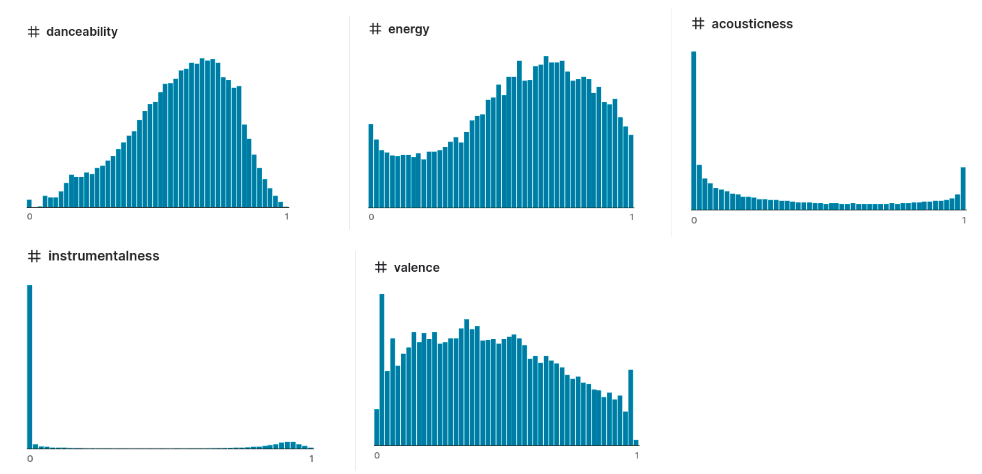
\includegraphics[width=\textwidth]{images/feature-distribution-kaggle.png}
      \caption{Distribution of audio features in the Spotify Audio Features Kaggle dataset.}
      \label{fig:audio-features-distribution-kaggle}
\end{figure}




\section{Experiments}

We trained three commonly used machine learning models to predict Spotify audio features from Last.fm tags by using the Last.fm Single-user dataset.
Considering that predicting the audio feature values is a regression problem, we tested the following models:

\begin{itemize}
      \item Boosted tree regressor \cite{xgboost}
      \item Bayesian Ridge Regressor \cite{bayesian}
      \item GPT-2 model (fine-tuning) \cite{radford2019language}
\end{itemize}


The \emph{Boosted tree regressor} is a specific implementation of the \emph{XGBoost} algorithm for regression tasks.
This algorithm is an ensemble learning technique that combines simple multiple decision trees to
create a stronger predictive model.
This model has proved to be a powerful solution for classification and regression problems on high-dimensional, structured data.
\textcolor{red}{REF}

The \emph{Bayesian Ridge regressor} is a regression model that combines the principles of Bayesian statistics with ridge regression.
Compared to linear regression, which assumes that the model estimated parameters have a deterministic value, the Bayesian Ridge regressor treats the model coefficients as variables with a prior distribution.
By incorporating prior distributions into the learning process, the model is able to capture uncertainty.
The ridge regression technique enables the model to handle noisy, collinear, structured data.

The \emph{GTP-2} model is a transformer model.
Transformers are a type of neural network architecture that has been widely used in natural language processing (NLP) tasks,
such as text generation and question answering.
GPT-2 has been trained on a large corpus of text, and typically used as a language model to generate text that resembles human-written language.
However, in this study we have experimented with GPT-2 as a regressor.
Rather than retraining the model from scratch, we have fine tuned the model to behave as a regressor and  predict Spotify audio features.
The basic idea behind this approach is to feed a string of concatenated Last.fm tags as input to the GPT-2 model, and then use the model's output as the predicted value of a specific Spotify audio feature.


\subsection{Last.fm Tags Input Format}

The preceding models require specific input formats.
Therefore, we tested different input formats.

Each individual sample in the dataset corresponds to a unique track,
and contains the list of Last.fm tag-count tuples (e.g. \verb|[(electronic, 100), (dance, 45), ...]|)
and the values of Spotify audio features.
Before experimenting with machine learning models, we prepared the data in a number of different formats,
each one suitable for specific models.


\subsubsection{Tabular}
With this format, the Last.fm tags are represented as a table.
Each tag is defined by a column and each cell contains the count value of a tag for a track.
A cell is 0 if a tag is missing for a track.

Counting the total amount of Last.fm tags in the user collection resulted, initially, in more than five million tags.
We quickly confirmed that building a tabular data set, in which every row contains millions of columns (Last.fm tags)
was doable, but presented scalability problems.
In addition to scalability limitations, classic machine learning models might not take advantage of using the full dataset.
These models might even perform poorly if too many input features are provided.
The reason for this is spurious relations or redundancy  between input features.
Models might find relations that are not real, and latent, redundant variables might be accountable multiple times, which creates a bias in the output.
Feature subject selection aims at solving these problems.

% For example, a Bayesian model might provide low-quality results of provided with variables that are not conditionally independent.

Therefore, we reduced the number of tags by picking a subset of the most relevant tags.

The reduction algorithm uses a basic data aggregation algorightm: group the data by tag, aggregate by summing the \emph{count} values for each tag,
order by the aggregated count, and finally select the top-$K$ items of the ranking.

We generated three versions of the dataset, with different values of $K$: 100, 1,000 and 10,000.

We consider this reduction approach an initial approach.
For this particular aspect, dimensionality reduction algorithms, such as PCA, are good candidates for future work.

After selecting the top-$K$ tags, the input data passed was formatted in tabular format, as follows:

\begin{itemize}
      \item Given that $Tags_{K}$ is the set of most $K$ frequent Last.fm tags in the user listening history
            and, where each $tag \in Tags_{K}$.
      \item Given that $Audio$ is the set of Spotify audio features, where each $feat \in Audio$.
      \item For each $track$:
      \begin{itemize}
            \item $X_{track},_{tag}$ is the strengh of $tag$ for $track$. This value is in the $0-100$ range.
            \item $y_{track},_{feature}$ is the value of the audio feature $y$ for $track$.
      \end{itemize}
\end{itemize}

An example of this data format is provided in table \ref{tabular_tags_format}.

\begin{table}[h]
      \begin{center}
      \begin{minipage}{\textwidth}
      \caption{Tabular data format for Last.fm tags in XGBoost and Bayesian regressors}\label{tabular_tags_format}%
      \begin{tabular}{@{}lllllll@{}}
      \toprule
      Track                         & $X_{electronic}$ & $X_{ambient}$ & $X_{\dots}$ & $y_{energy}$ & $y_{valence}$ & $y_{\dots}$ \\
      \midrule
      Massive Attack - Blue Lines   & 62               & 6             &  \dots      & 0.496        & 0.947         & \dots  \\
      The Beta Band - Squares       & 40               & 3             &  \dots      & 0.446        & 0.507         & \dots  \\
      \dots                         & \dots            & \dots         &  \dots      & \dots        & \dots         & \dots  \\
      \botrule
      \end{tabular}
      \end{minipage}
      \end{center}
\end{table}

When generating training data by track, the tabular formats present sparsity problems.

For tabular representations, we need to defined a fixed set of columns as tags.
For most of tracks, most columns are 0.

The sparsity of a matrix is the number of zero-valued elements divided by the total number of elements
(e.g., m * n for an m * n matrix) is called the sparsity of the matrix.


\subsubsection{Tabular Tokens}

Tags are converted to text tokens. Columns represent token positions, and cells contain the token at a particular position, for a track.
To tokenize tags, we have used the GTP-2 tokenizer.

Tokenizers are crucial elements in the preprocessing of text data.
A tokenizer dissects a piece of text into smaller units, called tokens.
These tokens can be words, subwords, or even syllables or characters.

When breaking down the text into tokens, the tokenizer assigns a unique numerical identifier to each token.
This IDs are based on the vocabulary that the tokenizer has been trained on.
For example, when the tokenizer processes the \verb|"Hello world"| string, the Hello token might be assigned to ID \verb|123|
and the world token might be assigned to ID \verb|34534|.
The result of tokenizing \verb|Hello world| would be \verb|[123, 34534]|.

Note that, although tokenizers are most commonly used in combination with transformer models, in this paper we test the possiblity of using theorem
to preproccess data passed to Bayesian an Tree models.

Because the tokenizer requires a string as input, we have converted the set of tags for each track into a string.
To \emph{stringify} the tags, we have concatenated tags with multiple strategies:

\begin{itemize}
      \item Ordering by count: \verb|"rock, pop"|.
      \item Including tag count: \verb|"rock 2, pop 1"|.
      \item Duplicating each tag $count$ times: \verb|"rock rock, pop"|.
\end{itemize}


In this particular case, the $X$ values of the tabular input data are tokens.
These tokens are obtained from passing the string of concatenated Last.fm tags through the GPT-2 tokenizer,
as the following procedure explains:

\begin{itemize}
      \item Given that $X_L$ is the token vocabulary, where $L$ is the maximum vocabulary length.
      \item Given that $Audio$ is the set of Spotify audio features, where each $feat \in Audio$.
      \item For each $track$:
      \begin{itemize}
            \item $X_{track},_{n}$ is token found at position $n$, after tokenizing the tags string.
            \item $y_{track},_{feature}$ is the value of the audio feature $y$ for $track$.
      \end{itemize}
\end{itemize}

An example of this data format is provided in table \ref{tabular_token_format}.

\begin{table}[h]
      \begin{center}
      \begin{minipage}{\textwidth}
      \caption{Tabular data format for tokens in XGBoost and Bayesian regressors}\label{tabular_token_format}%
      \begin{tabular}{@{}llllllll@{}}
      \toprule
      Track                         & $X_{0}$ & $X_{1}$ & $X_{2}$ & $X_{\dots}$ & $y_{energy}$ & $y_{valence}$ & $y_{\dots}$ \\
      \midrule
      Massive Attack - Blue Lines   & 101     & 5099    & 6154    &  \dots      & 0.496        & 0.947         &  \dots  \\
      The Beta Band - Squares       & 101     & 4522    & 2600    &  \dots      & 0.446        & 0.507         &  \dots  \\
      \dots                         & \dots   & \dots   & \dots   &  \dots      & \dots        & \dots         &  \dots  \\
      \botrule
      \end{tabular}
      \end{minipage}
      \end{center}
\end{table}

Similarly to the tags tabular format, we also defined fixed values for the number of columns: 10, 1,000, and 10,000.

The two tabular formats, with tags and tokens, were tested on the Naive Bayes and the Boosted tree regressors.


\subsection{Text Strings}

When using transformer models, the input data is a string.
We must represent the Last.fm tags, which are defined as $(tag, count)$ tuples, as strings.
To this end, we applied the same three transformations used in the tabular tokens formats,
concatenate the tags by ordering by count, by including the tag count, and by duplicating the tags.

After converting to a string, the formal definition of the input data is as follows:

\begin{itemize}
      \item Given that $X$ is tags represented as text.
      \item Given that $Audio$ is the set of Spotify audio features, where each $feat \in Audio$.
      \item For each $track$:
      \begin{itemize}
            \item $X_{track},_{n}$ is set of tags for $track$, encoded as a single string.
            \item $y_{track},_{feature}$ is the value of the audio feature $y$ for $track$.
      \end{itemize}
\end{itemize}

An example of this data format is provided in table \ref{text_format}.

\begin{table}[h]
      \begin{center}
      \begin{minipage}{\textwidth}
      \caption{Text data format for GPT-transformer. In this particular case, the tags have been concatenated by ordering by tag count}\label{text_format}%
      \begin{tabular}{@{}lllll@{}}
      \toprule
      Track                         & $X$                                   & $y_{energy}$ & $y_{valence}$ & $y_{\dots}$ \\
      \midrule
      Massive Attack - Blue Lines   & "hip hop, chill, bristol, \dots"      & 0.496        & 0.947         & \dots  \\
      The Beta Band - Squares       & "alternative rock, folk, \dots"       & 0.446        & 0.507         & \dots \\
      \dots                         & \dots                                 & \dots        & \dots         & \dots  \\
      \botrule
      \end{tabular}
      \end{minipage}
      \end{center}
\end{table}




% \subsection{Boosted Tree Regressor}

% We configured the boosted tree regressor model with the training parameters listed in table \ref{table_xgboost_training_params}.

% \begin{table}[h!]
%       \begin{center}
%       \begin{minipage}{174pt}
%       \caption{Training parameters for XGBoost regressor}\label{table_xgboost_training_params}%
%       \begin{tabular}{@{}llll@{}}
%       \toprule
%       Parameter               & Value \\
%       \midrule
%       objective               & reg:squarederror  \\
%       base score              & 0.5 \\
%       booster                 & gbtree  \\
%       colsample bylevel       & 1 \\
%       colsample bynode        & 1 \\
%       colsample bytree        & 1 \\
%       gamma\footnotemark[1]   & 0 \\
%       learning rate           & 0.300000012 \\
%       max delta step          & 0 \\
%       max depth               & 6 \\
%       min child weight        & 1 \\
%       estimators              & 200  \\
%       n jobs                  & 12  \\
%       num parallel tree       & 1 \\
%       predictor               & auto  \\
%       random state            & 0 \\
%       reg alpha               & 0 \\
%       reg lambda              & 1 \\
%       scale pos weight        & 1 \\
%       subsample               & 2 \\
%       tree method             & auto  \\
%       \botrule
%       \end{tabular}
%       \footnotetext[1]{Minimum loss reduction required to make a further partition on a leaf node of the tree.}
%       \end{minipage}
%       \end{center}
% \end{table}


% \subsection{Naive Bayes Regressor}

% The Naive Bayes Regressor, and in particular, Bayesian Ridge, is the model used for regression in this case.

% % COMMENT copied FROM BayesianRidge source code
% % https://github.com/scikit-learn/scikit-learn/blob/9aaed4987/sklearn/linear_model/_bayes.py#L24
% %
% %     There exist several strategies to perform Bayesian ridge regression. This
% %     implementation is based on the algorithm described in Appendix A of
% %     (Tipping, 2001) where updates of the regularization parameters are done as
% %     suggested in (MacKay, 1992). Note that according to A New
% %     View of Automatic Relevance Determination (Wipf and Nagarajan, 2008) these
% %     update rules do not guarantee that the marginal likelihood is increasing
% %     between two consecutive iterations of the optimization.

% The training parameters are listed in table \ref{table_bayesian_training_params}.

% \begin{table}[h]
%       \begin{center}
%       \begin{minipage}{174pt}
%       \caption{Training parameters for XGBoost regressor}\label{table_bayesian_training_params}%
%       \begin{tabular}{@{}llll@{}}
%       \toprule
%       Parameter                     & Value \\
%       \midrule
%       Maximum iterations            & 300   \\
%       Tolerance\footnotemark[1]     & \num{1e-03} \\
%       alpha 1                       & \num{1e-06} \\
%       alpha 2                       & \num{1e-06} \\
%       lambda 1                      & \num{1e-06} \\
%       lambda 2                      & \num{1e-06} \\
%       \botrule
%       \end{tabular}
%       \footnotetext[1]{Tolerance for the stopping criteria.}
%       \end{minipage}
%       \end{center}
% \end{table}




\subsection{Experiments Execution and Results}

Table \ref{table:experiment_results} summaries the experiment results.
The table provides RMSE values for each experiment.


% INFO - Training Set: (8654, 14)
% INFO - Validation Set: (2164, 14)
% INFO - Test Set: (2705, 14)

% TRAINING STATS
% Num examples = 8654
% Num Epochs = 10
% Instantaneous batch size per device = 10
% Total train batch size (w. parallel, distributed & accumulation) = 10
% Gradient Accumulation steps = 1
% Total optimization steps = 8660
% Number of trainable parameters = 124441344


\begin{table}[h!]
      \begin{center}
      \begin{minipage}{\textwidth}
      \caption{Experiment results. Cells values correspond to the RMSE value.}\label{table:experiment_results}%
      \begin{tabular}{@{}lllllll@{}}
      \toprule
      M         & Input format                        & Danceab...       & Acoustic...    & Energy          & Valence         & Instrumen... \\
      \midrule
      Base      &                                     & 0.276            & 0.438           & 0.329          & 0.395           & 0.541          \\
      \midrule
      Bayes     & 100 tags\footnotemark[1]            & 0.159            & 0.261           & 0.197          & 0.243           & 0.307          \\
      Bayes     & 1000 tags                           & 0.153            & 0.253           & 0.190          & 0.237           & 0.299          \\
      Bayes     & 10000 tags                          &\textbf{0.152}    &\textbf{0.251}   &\textbf{0.189}  &\textbf{0.236}   &\textbf{0.297}  \\
      Bayes     & 100 tokens D\footnotemark[2]        & 0.307            & 0.307           & 0.238          & 0.281           & 0.383          \\
      Bayes     & 10000 tokens D                      & 0.359            & 0.507           & 0.394          & 0.479           & 0.613          \\
      Bayes     & 1000 tokens D                       & 0.201            & 0.315           & 0.249          & 0.248           & 0.399          \\
      Bayes     & 100 tokens O\footnotemark[3]        & 0.191            & 0.305           & 0.237          & 0.282           & 0.376          \\
      Bayes     & 1000 tokens O                       & 0.237            & 0.343           & 0.276          & 0.339           & 0.428          \\
      Bayes     & 10000 tokens O                      & 0.237            & 0.343           & 0.276          & 0.339           & 0.428          \\
      Bayes     & 100 tokens TC\footnotemark[4]       & 0.191            & 0.304           & 0.236          & 0.281           & 0.380          \\
      Bayes     & 1000 tokens TC                      & 0.202            & 0.320           & 0.247          & 0.248           & 0.404          \\
      Bayes     & 10000 tokens TC                     & 0.234            & 0.341           & 0.274          & 0.321           & 0.430          \\
      \midrule
      Tree      & 100 tags                            & 0.154            & 0.257           & 0.188          & 0.240           & 0.302          \\
      Tree      & 1000 tags                           & 0.149            &\textbf{0.249}   & 0.184          & 0.236           & 0.291          \\
      Tree      & 10000 tags                          &\textbf{0.148}    & 0.250           &\textbf{0.181}  &\textbf{0.235}   &\textbf{0.290}  \\
      Tree      & 100 tokens D                        & 0.274            & 0.274           & 0.212          & 0.256           & 0.330          \\
      Tree      & 1000 tokens D                       & 0.173            & 0.278           & 0.215          & 0.220           & 0.339          \\
      Tree      & 10000 tokens D                      & 0.172            & 0.276           & 0.217          & 0.266           & 0.342          \\
      Tree      & 100 tokens O                        & 0.179            & 0.294           & 0.225          & 0.271           & 0.350          \\
      Tree      & 1000 tokens O                       & 0.182            & 0.294           & 0.224          & 0.270           & 0.353          \\
      Tree      & 10000 tokens O                      & 0.182            & 0.294           & 0.225          & 0.267           & 0.353          \\
      Tree      & 100 tokens TC                       & 0.172            & 0.280           & 0.211          & 0.262           & 0.342          \\
      Tree      & 1000 tokens TC                      & 0.174            & 0.282           & 0.215          & 0.220           & 0.344          \\
      Tree      & 10000 tokens TC                     & 0.175            & 0.281           & 0.214          & 0.270           & 0.345          \\
      \midrule
      GPT       & Duplicated\footnotemark[5]          & 0.157            & 0.244           & 0.193          & 0.245           & 0.322          \\
      GPT       & Ordered\footnotemark[6]             & 0.149            & \textbf{0.237}  & 0.188          & 0.235           & \textbf{0.297}          \\
      GPT       & Tags,Counts\footnotemark[7]         & \textbf{0.145}   & \textbf{0.237}  & \textbf{0.187} & \textbf{0.233}  & 0.301          \\

      \botrule
      \end{tabular}
      \footnotetext[1]{Tags in tabular format. Given $(rock, 3)$, the cell in the $rock$ column contains \verb*|3|.}
      \footnotetext[2]{Duplicated tokens in tabular format. Tags $(rock, 3), (pop, 2)$, are converted to the \verb*|"rock, rock, rock, pop, pop"| string,
      which a tokenizer converts to the list of input tokens (e.g. \verb*|[101,1005,16588,1005,2531, ...]|).
      These tokens are passed to the model in tabular format. Columns are $token_1$, $token_2$, $...$, $token_N$.}
      \footnotetext[3]{Ordered tokens in tabular format. Tags $(rock, 3), (pop, 2)$, are converted to the \verb*|"rock, pop"| string,
      which a tokenizer converts to the list of input tokens (e.g. \verb*|[101,1005,16588,1005,2531, ...]|).
      These tokens are passed to the model in tabular format. Columns are $token_1$, $token_2$, $...$, $token_N$.}
      \footnotetext[4]{Tokens in tabular format from tags and counts. Tags $(rock, 3), (pop, 2)$, are converted to the \verb*|"'rock' 3, 'pop' 2"| string,
      which a tokenizer converts to the list of input tokens (e.g. \verb*|[101,1005,16588,1005,2531, ...]|).
      These tokens are passed to the model in tabular format. Columns are $token_1$, $token_2$, $...$, $token_N$.}
      \footnotetext[5]{String. Given tags $(rock, 3), (pop, 2)$, input is formatted as \verb*|"rock, rock, rock, pop, pop"|.}
      \footnotetext[6]{String. Given tags $(rock, 3), (pop, 2)$, input is formatted as \verb*|"rock, pop"|.}
      \footnotetext[7]{String. Given tags $(rock, 3), (pop, 2)$, input is formatted as \verb*|"'rock' 3, 'pop' 2"|.}
      \end{minipage}
      \end{center}
\end{table}

\subsubsection{Results for Tabular Data Models}

\begin{figure}[h!]
      \centering
      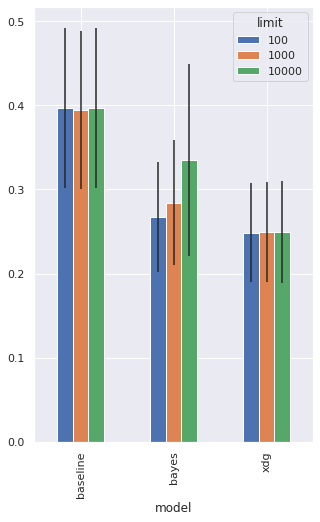
\includegraphics[width=0.5\textwidth]{images/rmse_by_model_and_limit.png}
      \caption{RMSE mean and standard deviation by model and tags/tokens limit.}
      \label{fig:rmse_by_model_and_limit}
\end{figure}


\begin{figure}[h!]
      \centering
      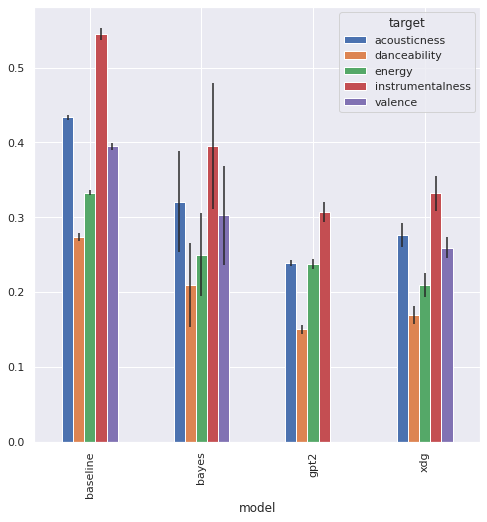
\includegraphics[width=0.7\textwidth]{images/rmse_by_model_and_feature.png}
      \caption{RMSE mean and standard deviation by model and audio feature.}
      \label{fig:rmse_by_model_and_feature}
\end{figure}


\begin{figure}[h!]
      \centering
      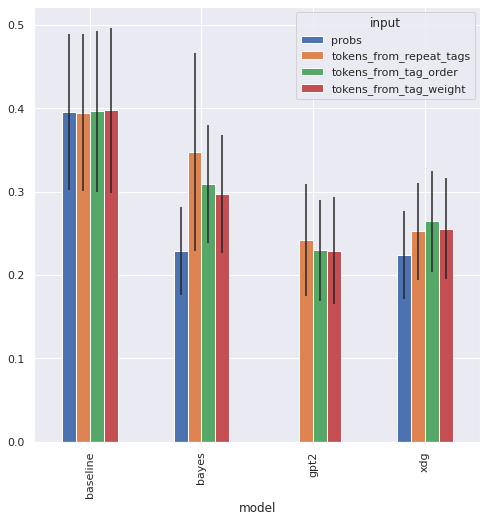
\includegraphics[width=0.7\textwidth]{images/rmse_by_model_and_input.png}
      \caption{RMSE mean and standard deviation by model and input type (tag probablities or tokens).}
      \label{fig:rmse_by_model_and_input}
\end{figure}


\begin{figure}[h!]
      \centering
      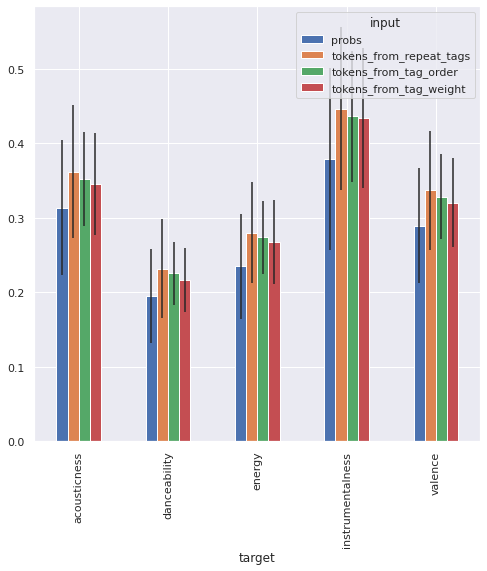
\includegraphics[width=0.7\textwidth]{images/rmse_by_feature_and_input.png}
      \caption{RMSE mean and standard deviation by audio feature and input type (tag probablities or tokens).}
      \label{fig:rmse_by_feature_and_input}
\end{figure}

\section{Conclusions}

In general, we believe that this novel approach that has the potential to benefit both listeners and researchers.
By combining subjective user-generated tags with objective audio features,
we can gain new insights into the complex relationship between perception and audio signal in music.

Our approach also presents limitations.
One limitation is the assumption of a strong relationship between Last.fm tags and Spotify features, which may not be true in all cases.
Future work could explore other sources of input values, possibly related to the user context, to improve the accuracy of the predictions.

Track mapping between Last.fm and Spotify is another opportunity for research and improvement.
Although Last.fm provides the MusicBrainz unique identifier, but Spotify does not provide this value.
The mapping was performed by using the track artist and name, but this approach resulted on about 30\% of the tracks not found on Spotify.



\textcolor{red}{TODO}


\section{Acknowledgments}

\textcolor{red}{TODO}



%%===========================================================================================%%
%% If you are submitting to one of the Nature Portfolio journals, using the eJP submission   %%
%% system, please include the references within the manuscript file itself. You may do this  %%
%% by copying the reference list from your .bbl file, paste it into the main manuscript .tex %%
%% file, and delete the associated \verb+\bibliography+ commands.                            %%
%%===========================================================================================%%

\bibliography{bibliography}% common bib file
%% if required, the content of .bbl file can be included here once bbl is generated
%%\input sn-article.bbl

%% Default %%
%%\input sn-sample-bib.tex%

\end{document}
